\documentclass{article}
\usepackage{listings}
\usepackage{graphicx}
\usepackage{float}
\usepackage{fontspec}
\setmainfont{Ubuntu}
\setsansfont{Ubuntu}% Ubuntu as sans - use \sffamily or \textsf{} as normal
\setmonofont{JetBrainsMono Nerd Font Mono}% Ubuntu Mono as 'typewriter' - use \ttfamily or \texttt{}
\usepackage[a4paper,
            bindingoffset=0.2in,
            left=1cm,
            right=1cm,
            top=1in,
            bottom=1in,
            footskip=.25in]{geometry}
\usepackage{hyperref}
\hypersetup{
    colorlinks, citecolor=black, filecolor=black,
    linkcolor=black, urlcolor=black
}
\usepackage{xcolor}
\definecolor{mygreen}{rgb}{0.05,0.15,0.11}
\definecolor{mygray}{rgb}{0.9,0.9,0.9}
\definecolor{mymauve}{rgb}{0.58,0,0.82}
\lstset{
  % backgroundcolor=\color{mygray}, 
  basicstyle=\ttfamily,
  breakatwhitespace=false,
  breaklines=true,
  % commentstyle=\color{darkgray},
  keepspaces=true,
  keywordstyle=\bfseries,
  morekeywords={*,...},
  showspaces=false,
  showstringspaces=false,
  showtabs=false,
  % stringstyle=\color{blue},
  tabsize=4,
  % numbers=left,
  rulecolor=\color{black},
  postbreak=\mbox{\textcolor{red}{$\hookrightarrow$}\space}
}

\begin{document}

\pagenumbering{gobble}
{\centerline{\bfseries \Huge Assignment 8}}

\section*{Question 1}
Write a JavaScript function to get the current date.
\subsection*{Code}
\lstinputlisting[language=html]{1/index.html}
\subsection*{Output}
\begin{figure}[H]
    \centering
    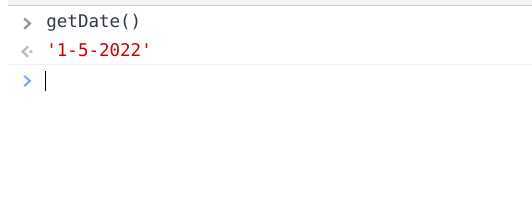
\includegraphics[width=10cm]{1/out.png}
\end{figure}

\newpage
\section*{Question 2}
Write a JavaScript function to get the number of days in a month.
\begin{lstlisting}
Test Data :
    console.log(getDaysInMonth(1, 2012));
    console.log(getDaysInMonth(2, 2012));
    console.log(getDaysInMonth(9, 2012));
    console.log(getDaysInMonth(12, 2012));
Output :
    31
    29
    30
    31
\end{lstlisting}
\subsection*{Code}
\lstinputlisting[language=html]{2/index.html}
\subsection*{Output}
\begin{figure}[H]
    \centering
    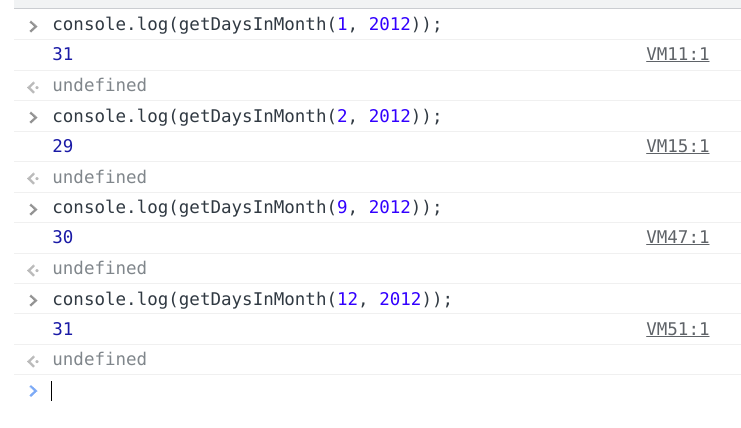
\includegraphics[width=10cm]{2/out.png}
\end{figure}

\newpage
\section*{Question 3}
Write a JavaScript function to get the month name from a particular date
\begin{lstlisting}
Test Data :
    console.log(month_name(new Date("10/11/2009")));
    console.log(month_name(new Date("11/13/2014")));
Output :
    "October"
    "November"
\end{lstlisting}
\subsection*{Code}
\lstinputlisting[language=html]{3/index.html}
\subsection*{Output}
\begin{figure}[H]
    \centering
    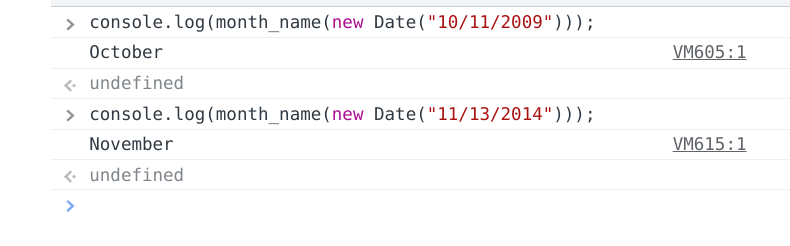
\includegraphics[width=10cm]{3/out.png}
\end{figure}

\newpage
\section*{Question 4}
Write a JavaScript program to display the current day and time in the
following format. \\
Sample Output : \\
Today is : Friday. \\
Current time is : 4 PM : 50 : 22 \\
\subsection*{Code}
\lstinputlisting[language=html]{4/index.html}
\subsection*{Output}
\begin{figure}[H]
    \centering
    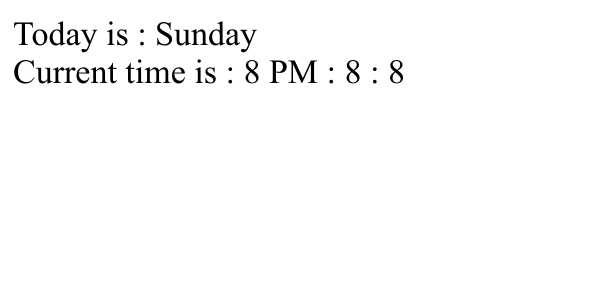
\includegraphics[width=10cm]{4/out.png}
\end{figure}

\newpage
\section*{Question 5}
Write a JavaScript program to get the current date. \\
Expected Output : \\
mm-dd-yyyy, mm/dd/yyyy or \\
dd-mm-yyyy, dd/mm/yyyy
\subsection*{Code}
\lstinputlisting[language=html]{5/index.html}
\subsection*{Output}
\begin{figure}[H]
    \centering
    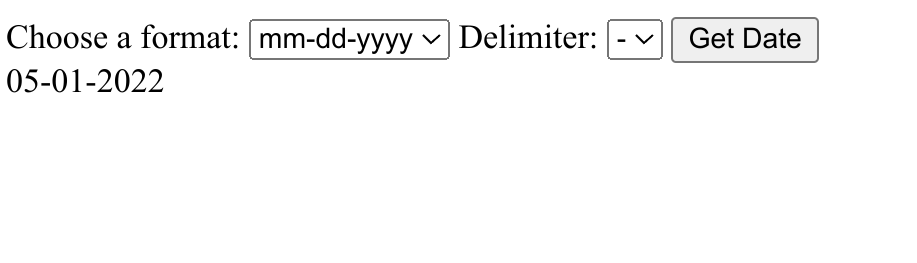
\includegraphics[width=10cm]{5/out.png}
\end{figure}

\newpage
\section*{Question 6}
Write a JavaScript function to get difference between two dates in days.
\begin{lstlisting}
Test Data :
    console.log(date_diff_indays('04/02/2014', '11/04/2014'));
    console.log(date_diff_indays('12/02/2014', '11/04/2014'));
Output :
    216
    -28
\end{lstlisting}
\subsection*{Code}
\lstinputlisting[language=html]{6/index.html}
\subsection*{Output}
\begin{figure}[H]
    \centering
    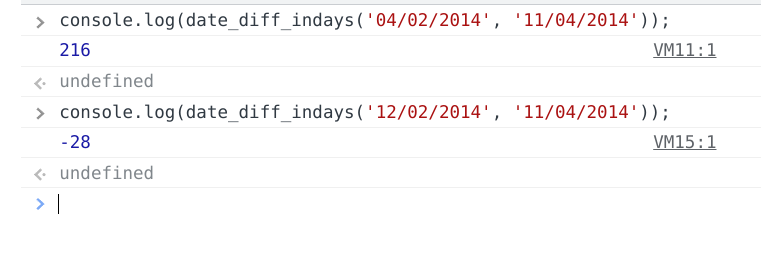
\includegraphics[width=10cm]{6/out.png}
\end{figure}

\end{document}
